
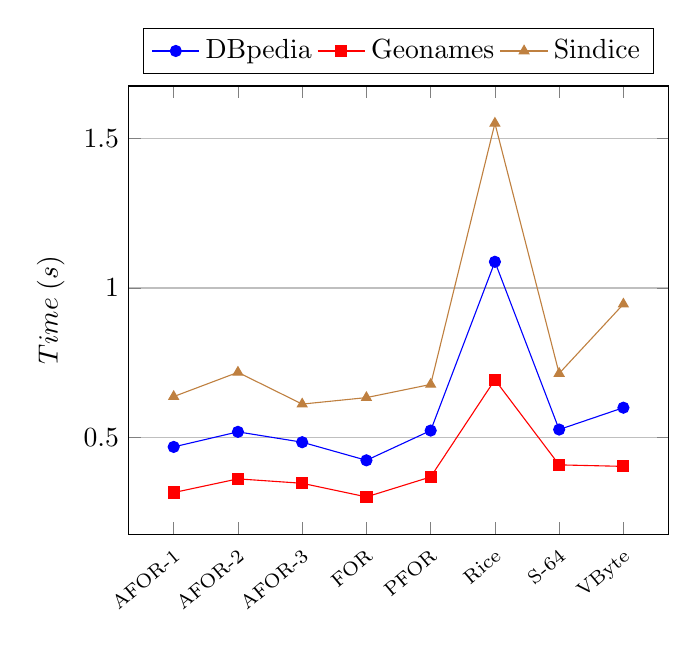
\begin{tikzpicture}
\begin{axis}[
ylabel=$Time \; (s)$,
x tick label style={font=\scriptsize, rotate=40, anchor=north east},
xtick={1,...,8},
xticklabels={AFOR-1, AFOR-2, AFOR-3, FOR, PFOR, Rice, S-64, VByte},
legend style={at={(0.5,1.13)}, anchor=north, legend columns=-1},
%ybar,
ymajorgrids=true,
%bar width=7pt,
]

\addplot[blue,mark=*]
coordinates {(1, 0.4692) (2, 0.5195) (3, 0.4849) (4, 0.4244) (5, 0.5238) (6, 1.0875) (7, 0.5272) (8, 0.6002)};
\addplot[red,mark=square*]
coordinates {(1, 0.3167) (2, 0.3625) (3, 0.3477) (4, 0.3022) (5, 0.3689) (6, 0.6936) (7, 0.4092) (8, 0.4042)};
\addplot[brown,mark=triangle*]
coordinates {(1, 0.6373) (2, 0.7183) (3, 0.6122) (4, 0.6339) (5, 0.6779) (6, 1.55) (7, 0.7146) (8, 0.946)};

\legend{DBpedia, Geonames, Sindice}

\end{axis}
\end{tikzpicture}

